%%%%%%%%%%%%%
%  Ch1 : Generalities  %
%%%%%%%%%%%%%

\chapter{Discrete systems}
	\section{Introduction}
		Vibrations are found on everything around us, trains, cars and even human body is subject to vibration. Its effects are disturbing because it causes fatigue, loss of performance, no comfort, ... As vibration source we can find the earthquakes, the interaction with road, the wind, the waves, ... The basic terminology for the course is:
		
		\begin{multicols}{3}
		\begin{itemize}
		\item[•] \textbf{The source} $F(\omega)$,\\
		this characterizes the dynamic forces
		\item[•] \textbf{The path} $H(\omega)$,\\
		this characterizes the structural dynamics
		\item[•] \textbf{The response} $X(\omega)$,
		such that $X(\omega)=H(\omega)F(\omega)$.
		\end{itemize}
		\end{multicols}
		
		Vibrations cause failure, loss of comfort and is harmful for precision operations. We try to suppress it by damping, isolation and structure design.\\
		
		We have two different approach for analysing a vibration problem. The one called \textbf{Signal analysis} or \textbf{Fourier analysis} deals with the case where we only have the response of the system to unknown forces. The one called \textbf{System analysis} or \textbf{Modal analysis} where we stimulate the system with known forces and measure the response, being able to find $H(s)$ (dynamic forces - transfer function of the system). \\
		
			\subsubsection{Basic notions}
			\begin{wrapfigure}[7]{l}{2.5cm}
			\vspace{-5mm}
			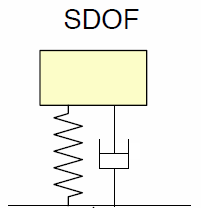
\includegraphics[scale=0.5]{ch1/1}
			\captionof{figure}{}
			\end{wrapfigure}			
			Three main forces are acting on bodies:
			
			\begin{itemize}
				\item[•] the one due to springs, proportional to the displacement: $F = kd $
				\item[•] the one due to dampers, proportional to the velocity: $F = cv$
				\item[•] the one due to the mass, proportional to acceleration: $F =ma$.
			\end{itemize}
			
			\ \\ Notice that we have one resonance frequency for each degree of liberty of each mass. \newpage
			
			\begin{wrapfigure}[8]{r}{4cm}
			\vspace{-8mm}
			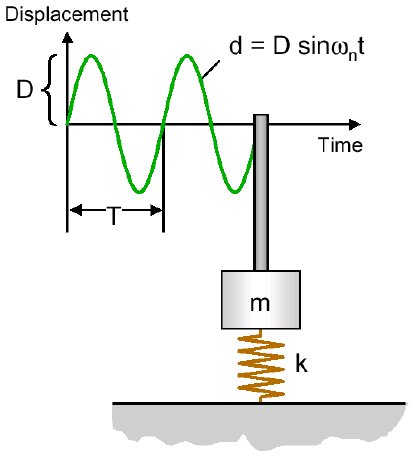
\includegraphics[scale=0.35]{ch1/2}
			\captionof{figure}{}
			\end{wrapfigure}		
			We can already get some definition, let's consider the free vibration assumed to be always in resonance. We can then define the \textbf{period of resonance} $T_n$, the \textbf{resonance frequency} $f_n = \frac{1}{T_n}$ and the \textbf{resonance pulsation}:
			\begin{equation}
			\omega _n = 2\pi f_n = \sqrt{\frac{k}{m}}.
			\end{equation}
			
			Notice that if we increase mass, the frequency decreases. 
			\\\\
			
			\begin{wrapfigure}[8]{l}{7cm}
			\vspace{-5mm}
			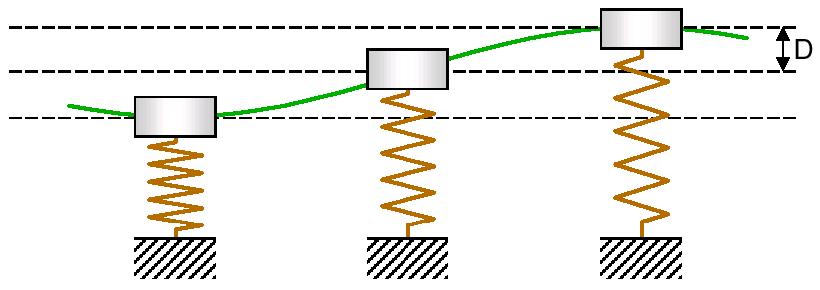
\includegraphics[scale=0.3]{ch1/3}
			\captionof{figure}{}
			\end{wrapfigure}
			Then we have the \textbf{energy transfer} between the kinetic energy and the potential energy. Indeed we see that velocity is null on extreme position and max when at the middle. This is written as:
			
			\begin{equation}
			\frac{1}{2} m V^2 = \frac{1}{2} kD^2
			\end{equation}
			
			where $V = 2\pi f_n D$. Replacing by this:
			
			\begin{equation}
			 m (2\pi f_n D)^2 = kD^2 \qquad \Rightarrow f_n = \frac{1}{2\pi}\sqrt{\frac{k}{m}}.
			\end{equation}
			
			We find a waited result. Now, let's show that \textbf{increasing damping reduces amplitudes over time}. Take the general newton equation for a linear free system and multiply by $\dot{x} (t)$:
			
			\begin{equation}
			m\ddot{x}\dot{x} + b\dot{x}\dot{x} + kx\dot{x} = 0 \qquad \Rightarrow \frac{d}{dt}\left( \frac{1}{2} m\dot{x}^2 + \frac{1}{2} kx^2 \right) = -b\dot{x}^2 \leq 0
			\end{equation}
			
	\section{Single degree of freedom oscillator}
		\begin{wrapfigure}[8]{r}{3.5cm}
			\vspace{-5mm}
			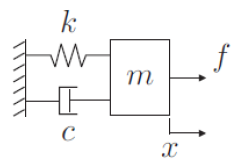
\includegraphics[scale=0.6]{ch1/4}
			\captionof{figure}{}
			\end{wrapfigure}
			Given the single degree system here, its free response is given by:
			
			\begin{equation}
			m\ddot{x}\dot{x} + b\dot{x}\dot{x} + kx\dot{x} = 0.
			\end{equation}
			
			We assume that this differential equation admits a solution of type $x = Ae^{st}$. We can then write the characteristic equation and its eigenvalues as:
			
			\begin{equation}
			ms^2 + cx + k = 0, \qquad s = - \frac{c}{2m} \pm j\sqrt{\frac{k}{m} -\frac{c^2}{4m^2}}.
			\end{equation}
			
			By defining two new quantity, the \textbf{natural pulsation} $\omega _n ^2 = \frac{k}{m}$ and the \textbf{damping ratio} $\xi$ such that $\xi \omega _n = \frac{c}{2m}$, we can rewrite:
			
			\begin{equation}
			s = - \xi \omega _n \pm j\omega _n \sqrt{1 -\xi ^2}.
			\end{equation}
			
			\begin{wrapfigure}[7]{l}{7.5cm}
			\vspace{-5mm}
			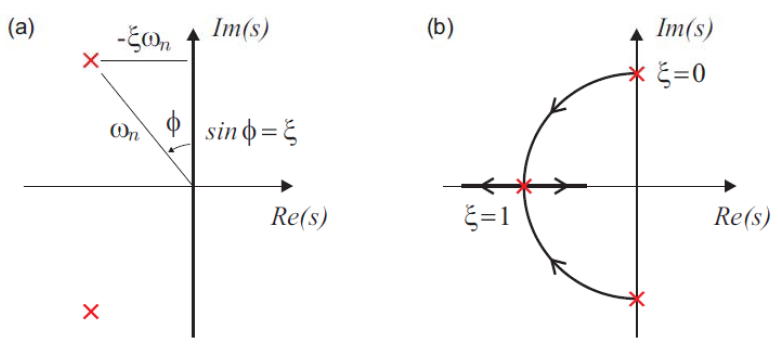
\includegraphics[scale=0.35]{ch1/5}
			\captionof{figure}{}
			\end{wrapfigure}
			We can introduce the \textbf{damping pulsation} $\omega _d = \omega _n \sqrt{1-\xi ^2}$. This explicitly makes appear the real and imaginary part of $s$ that we plot on a diagram. Notice that the norm and the angle of the complex number are $\omega _n$ and $\arcsin \xi$. \\
			
			The right figure is the \textbf{Nyquist diagram}. Last, the final expression for $x$ is:
			\begin{equation}
			x = e^{-\xi \omega _n t} \left( Ae^{j\omega _d t}+ Be^{-j\omega _d t} \right) = e^{-\xi \omega _n t} \left( A_1\cos (\omega _d t)+ B_1 \sin (\omega _d t) \right)
			\label{eq:1.8}
			\end{equation}
			where $A,B,A_1,B_1$ depends on initial conditions. 
			
			\subsubsection{Impulse response}
				\begin{wrapfigure}[9]{l}{2cm}
				\vspace{-5mm}
				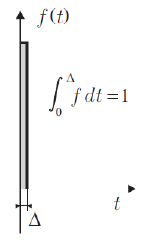
\includegraphics[scale=0.6]{ch1/6}
				\captionof{figure}{}
				\end{wrapfigure}
				Let's now apply an impulse on the system and let's analyse when it is applied during the infinitesimal time $\Delta$, given the initial conditions $x = 0, \dot{x}=0$. If we integrate the newton equation:
				\begin{equation}
				\int _0 ^\Delta m \ddot{x} \,dt = \int _0 ^\Delta f \,dt - \cancel{\int _0 ^\Delta c \dot{x}\,dt} - \cancel{\int _0 ^\Delta kx\,dt} = 1
				\end{equation}				 
				where the spring and damping forces cancel as they are finite (infinitesimal integral), the impulse integral =1 by definition. Taking the limit we find new initial conditions:
				
				\begin{wrapfigure}[8]{r}{3.5cm}
				\vspace{-5mm}
				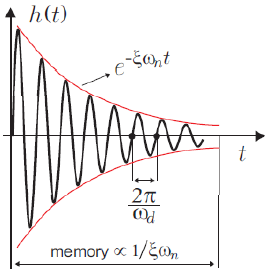
\includegraphics[scale=0.5]{ch1/7}
				\captionof{figure}{}
				\end{wrapfigure}
				\begin{equation}
				\lim _{\Delta \rightarrow 0} m\dot{x}(\Delta) = m\dot{x}(0^+) = 1  \qquad \Rightarrow x(0^+) = 0, \dot{x}(0^+) = \frac{1}{m}.
				\end{equation}

				The resolution of \eqref{eq:1.8} gives the \textbf{impulse response}:
				\begin{equation}
				x(t) = h(t) = \frac{1}{m\omega _d} e^{- \xi\omega _n t} \sin (\omega _d t)
\end{equation}				 

	\section{Convolution integral}
		\begin{wrapfigure}[8]{l}{4cm}
		\vspace{-5mm}
		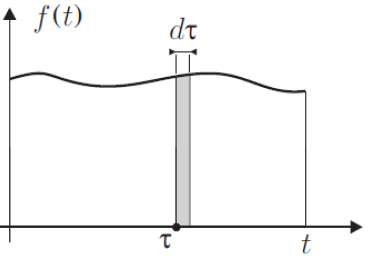
\includegraphics[scale=0.4]{ch1/8}
		\captionof{figure}{}
		\end{wrapfigure}
		Consider a transfer function $h(t)$ of a system and the decomposition shown on the figure. The output of the system will be computed with the convolution integral:
		
		\begin{equation}
		x = \int _0^t h(t-\tau)f(\tau) \, d\tau.
		\end{equation}
		
		where $h(t)$ is the \textbf{impulse response}. In particular, for a \textbf{causal} system:
		
		\begin{equation}
		x(t) = \int _{-\infty}^{\infty} h(t-\tau)f(\tau)\, d\tau = \int _{-\infty}^{\infty} h(\tau)f(t-\tau)\, d\tau = h(t)*f(t).
				\label{eq:1.13}
		\end{equation}	
		
		\subsection{Harmonic response}
			Consider an undamped system	to which we apply an harmonic force:
			
			\begin{equation}
			m \ddot{x} + kx = F e^{j\omega t}.
			\end{equation}
			
			By considering the Fourier transform $x(t) = X(\omega )e^{j\omega t}$, we get:
			
			\begin{equation}
			-\omega ^2 X(j\omega) + \frac{k}{m} X(j\omega) = \frac{F(j\omega)}{m} \qquad \Rightarrow X = \frac{F}{k} \frac{1}{1-(\omega / \omega)^2} = \frac{F}{k} D(\omega)
			\end{equation}
			
			where $D(\omega)$ is the \textbf{dynamic amplification}. For the damped case, we only have to know that $\xi \omega _n = c/2m$ and we get in the same way as previously:
			
			\begin{equation}
			X = \frac{F}{k}\frac{1}{1-(\omega / \omega)^2 + 2j\omega / \omega _n } = \frac{F}{k} D(\omega).
			\end{equation}
			
			The two dynamic amplifications are plotted on the figures below, the second on a Bode diagram where we can clearly see the \textbf{Quality factor} defined as $Q = 1/2\xi$. 
			
			\begin{center}
			\begin{minipage}{0.4\textwidth}
			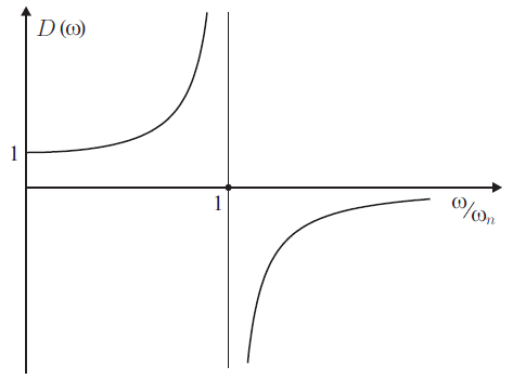
\includegraphics[scale=0.4]{ch1/9}
			\captionof{figure}{}
			\end{minipage}
			\begin{minipage}{0.4\textwidth}
			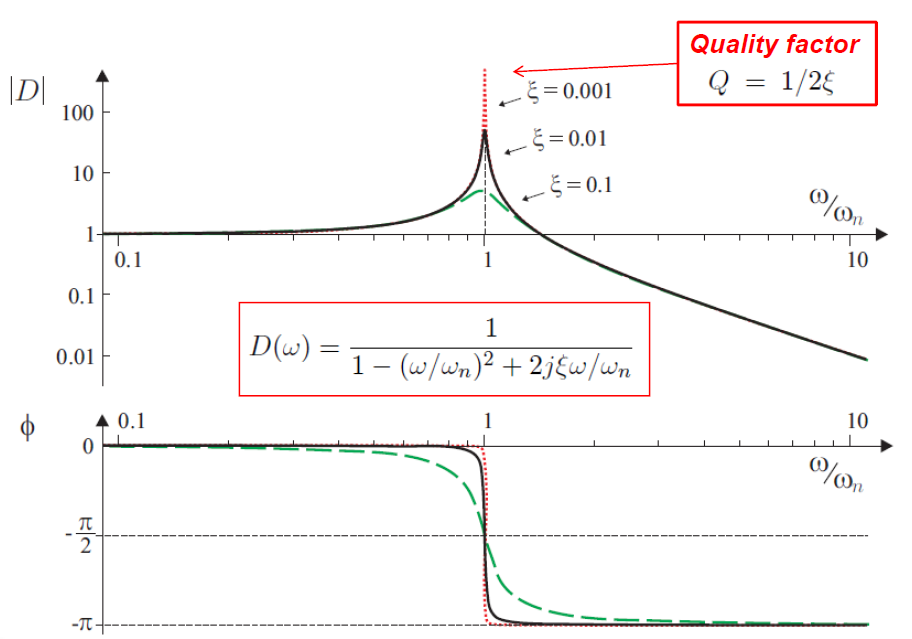
\includegraphics[scale=0.24]{ch1/10}
			\captionof{figure}{}
			\end{minipage}
			\end{center}
			
		\subsection{Frequency response function}
			Let's remember that the response is given by the convolution integral \eqref{eq:1.13}, where we will define now $h(t)$. Assuming the applied force to be harmonic $Fe^{i\omega t}$, then proceeding to the Fourier transform of x, we get:
			
			\begin{equation}
			Xe^{i\omega t} = \int _{-\infty}^\infty h(t)Fe^{i\omega (t-\tau)} \, d\tau \qquad \Rightarrow \frac{X(\omega)}{F(\omega)} = \int _{-\infty}^\infty h(t)e^{-i\omega \tau} \, d\tau = H(\omega)
			\end{equation}
			
			\begin{wrapfigure}[5]{l}{8cm}
			\vspace{-5mm}
			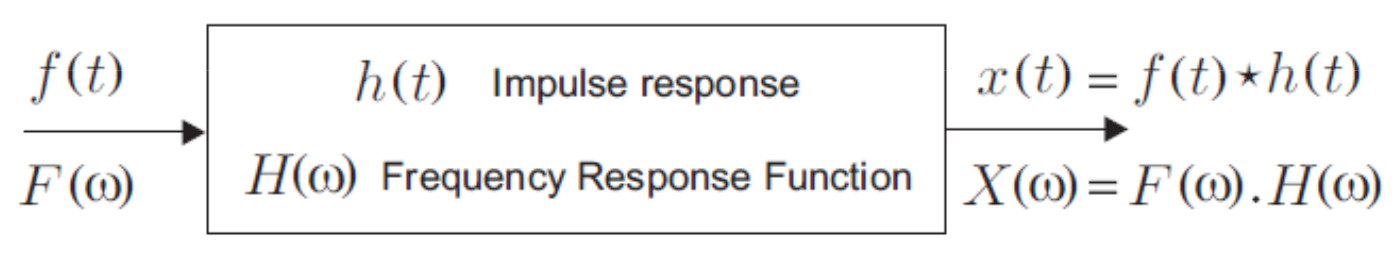
\includegraphics[scale=0.3]{ch1/11}
			\captionof{figure}{}
			\end{wrapfigure}
			where we end up with the fact that \textbf{the frequency response function is the Fourier transform of the impulse response}. We can thus avoid the convolution to have a simple multiplication after a Fourier transform. Here is also a useful theorem where $|F(\omega)/2\pi |$ is the \textbf{energy spectrum} of $f(t)$: 
			
			\begin{center}
			\theor{
			\textbf{Parseval theorem}
			\begin{equation}
			\int _{-\infty} ^\infty f^2(t) \, dt = \frac{1}{2\pi} \int _{-\infty} ^\infty |F(\omega)|^2 \, d\omega .
			\end{equation}						
			}
			\end{center}
			
		\subsection{Discrete Fourier Transform}
			Consider a signal x sampled in N samples, the equivalence of the continuous Fourier transform in discrete domain and the inverse transform are:
			
			\begin{center}
			\theor{
			\begin{equation}
			X_k = \sum _{n=0}^{N-1} x_n e^{- i \frac{2k\pi}{N}n} \qquad \mbox{and} \qquad X_n = \frac{1}{N}\sum _{k=0}^{N-1} X_k e^{i \frac{2k\pi}{N}n}
			\end{equation}
			}
			\end{center}
			
			The equivalent Parseval theorem is:
			
			\begin{equation}
			\sum _{n=0}^{N-1}|x_n|^2 = \frac{1}{N} \sum _{k=0}^{N_1} |X_k|^2
			\end{equation}
			
			And as last definition, we have the root-mean-square value defined as 
			\begin{equation}
			RMS = \sqrt{\frac{1}{N}\sum _{n=0}^{N-1}|x_n|^2} = \sqrt{\frac{1}{N^2}\sum _{k=0}^{N-1}|X_n|^2}
			\end{equation}
			
			\section{Transient response (Beat)}
				Consider an undamped oscillator excited by an harmonic force $F\cos \omega t$ and of impulse response:
				\begin{equation}
				h(t) = \frac{1}{m\omega _n} \sin \omega _nt 
 				\end{equation}
 				
 				Applying the convolution integral to this problem and integrating by part we find:
 				\begin{equation}
 				x(t) = \int _0 ^t F\cos (\omega t) h(t-/tau ) \, d\tau = \frac{F}{m} \frac{\cos (\omega t) - \cos (\omega _n t)}{\omega _n ^2 - \omega ^2} 
 				\end{equation}
 				
 				\begin{wrapfigure}[16]{l}{8cm}
				\vspace{-5mm}
				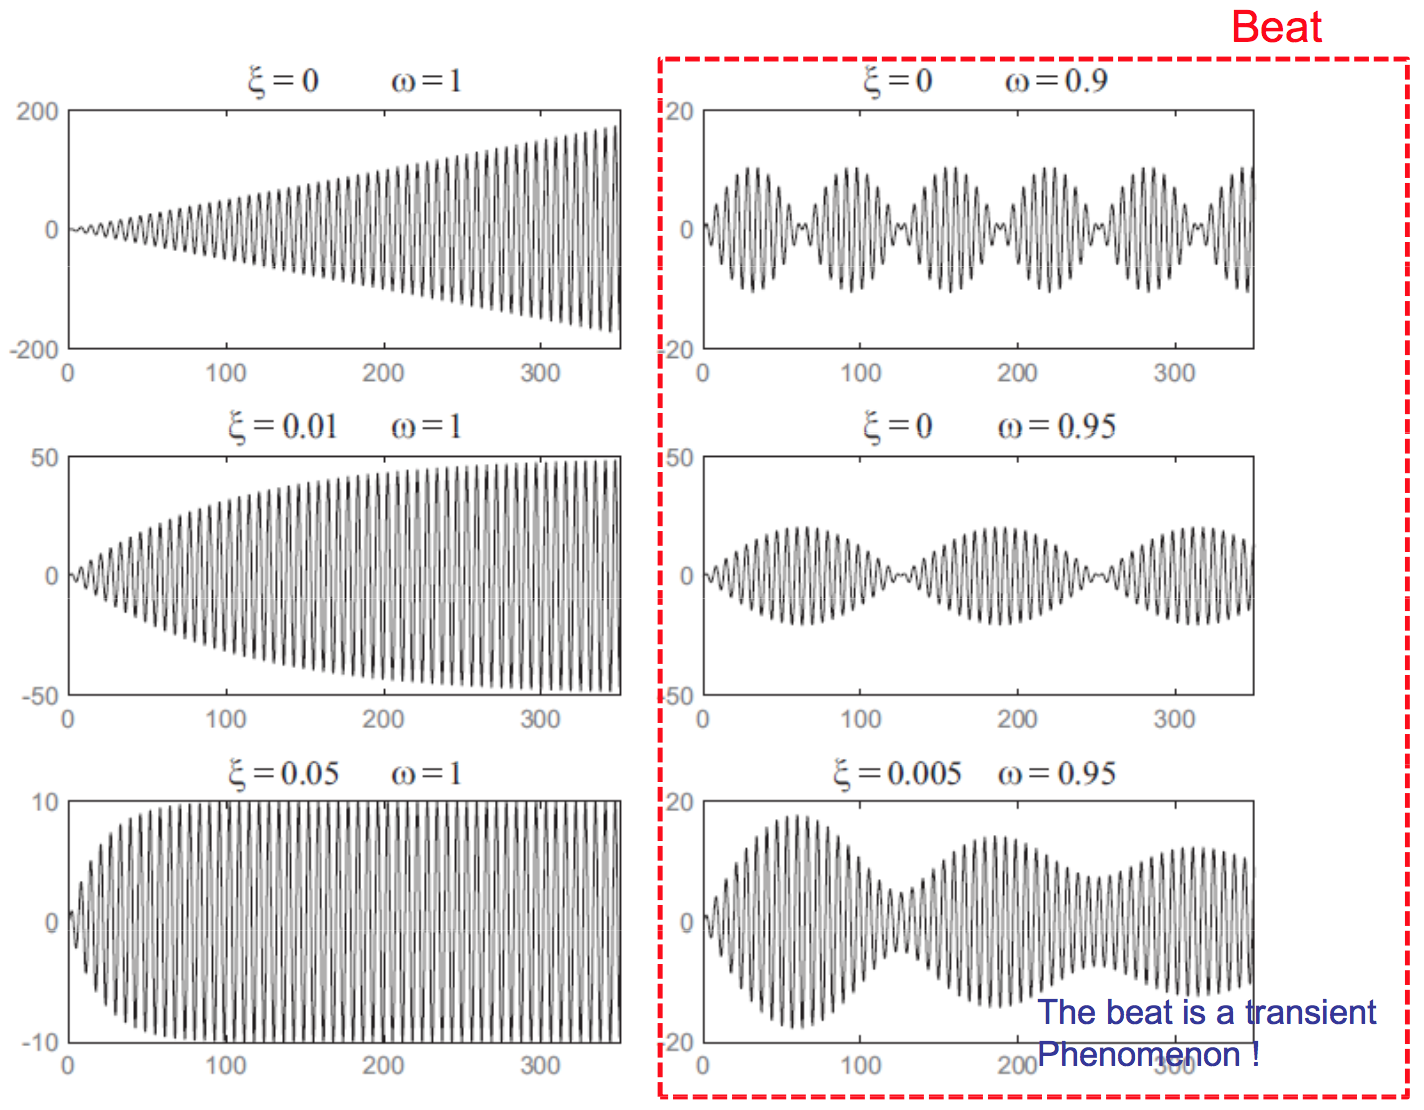
\includegraphics[scale=0.3]{ch1/12}
				\captionof{figure}{}
				\end{wrapfigure}
				By using Simpson's formula, defining $\omega + \omega _n = 2\omega _0$ and $\omega - \omega _n = 2\Delta$, we get:
 				
 				\begin{equation}
 				x(t) = \frac{F}{m} \frac{\sin (\omega _0t)\sin (\Delta t)}{2\omega _0 \Delta}
 				\end{equation}
 				
 				Remark that for $\Delta \rightarrow 0, \ \frac{\sin \Delta t}{\Delta} = t$. This term is called the \textbf{modulating function} as it grows the response amplitude while the other sinus is confined in $[-1,1]$. We get thus for resonance:
 				
 				\begin{equation}
 				x(t) = \frac{F}{m} \frac{\sin (\omega _nt)}{2\omega _n}	t.
				\end{equation} 				 
 				
 				The figure shows that the phenomenon known as beat is \textbf{in fact} a transient phenomenon. 
 				
 		\section{Multiple degree of freedom}
 			Before going throw the real subject, let's introduce what's the \textbf{state space model} (yes CSD). It consists in writing any differential equation in this form of first order equation:
 			
 			\begin{equation}
 			\dot{x} = A x+ Bu
 			\end{equation}
 			where A, B are matrices and x, u vectors. Let's apply this for an oscillator:
 			
 			\begin{equation}
 			\ddot{x} = \frac{f}{m} - 2\xi \omega _n - \omega _n^2 
 			\end{equation}
 			
 			We choose as state variable $x_1 = x$ and $x_2 = \dot{x}$, then we only have to rewrite the definition of $\dot{x}_1$ and $\dot{x}_2$ as:
 			
 			\begin{equation}
 			\left\{
 			\begin{array}{c}
 			\dot{x}_1\\
 			\dot{x}_2
 			\end{array}
 			\right\}
 			=
 			\left[
 			\begin{array}{cc}
 			0 & 1\\
 			-\omega _n ^2 & 2\xi \omega
 			\end{array}
 			\right]
 			\left\{
 			\begin{array}{c}
 			{x}_1\\
 			{x}_2
 			\end{array}
 			\right\}
 			+
 			\left\{
 			\begin{array}{c}
 			0\\
 			\frac{1}{m}
 			\end{array}
 			\right\}
 			f
 			\end{equation}
 			
 			\begin{wrapfigure}[16]{l}{9cm}
			\vspace{-5mm}
			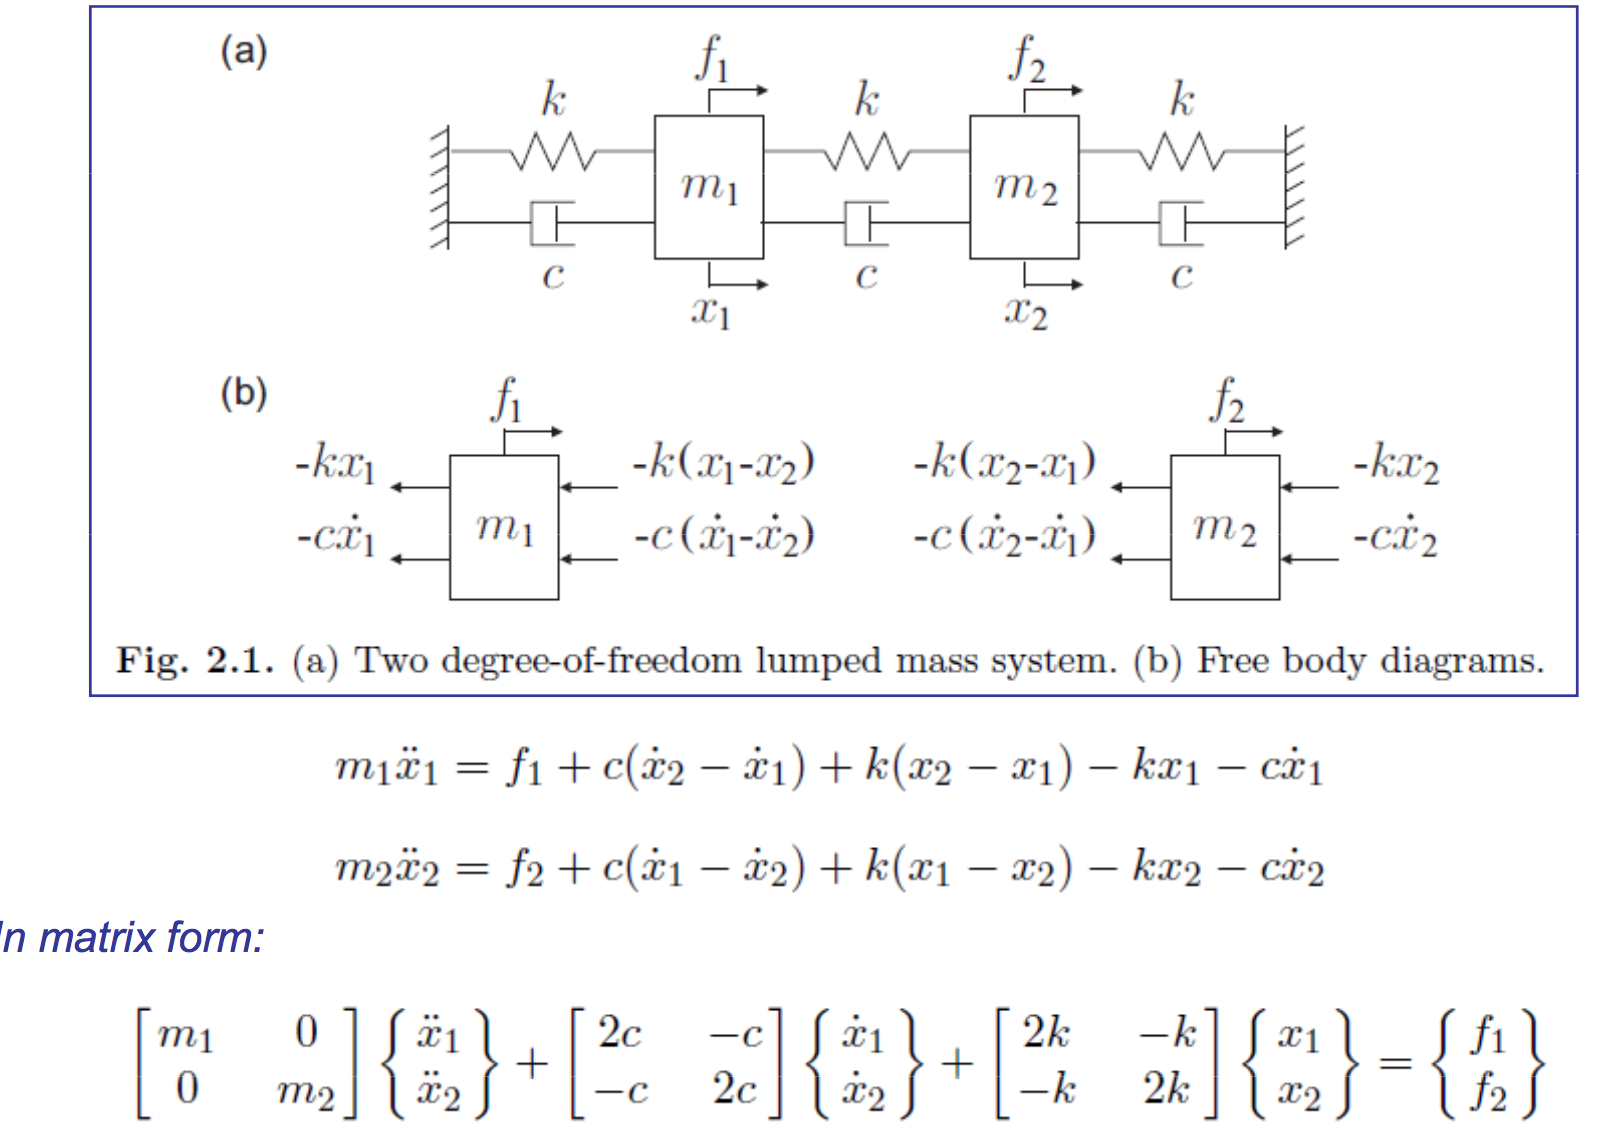
\includegraphics[scale=0.3]{ch1/13}
			\captionof{figure}{}
			\label{fig:1.13}
			\end{wrapfigure}
			Let's now look at the multiple degree case on \autoref{fig:1.13}. The first thing to do is to put everything in matrix form. We see that we have something in the form:
			
			\begin{equation}
				M\ddot x + C \dot{x} + Kx = f.
\end{equation}			 

			The matrices M, C, K are symmetric and semi-positive definite: $K = K^T$ and $x^TKx\geq 0, \ \forall x$. In particular, we can compute the kinetic energy and the strain energy as:
			
			\begin{equation}
			\frac{1}{2}\dot{x}^TM\dot{x} \qquad \mbox{and} \qquad \frac{1}{2} {x}^TK{x}
			\end{equation}
			
		\section{Eigenvalue problem}
			The method to solve this problem is to first consider the free response of the conservative system $(C=0)$: $M\ddot{x} + Kx = 0$. A non trivial solution exists if: 
			
			\begin{equation}
				(K+s^2M)\phi = 0
			\end{equation}
			
			The eigenvalues $s$ are solution of $\det (K+s^2M) = 0$ Because K and M are symmetric and semi-positive definite, the eigenvalues are purely imaginary: $s= \pm j\omega$, this gives:
			
			\begin{equation}
				(K-\omega _i M)\phi _i = 0
			\end{equation}
			
			where $\omega _i$ are the natural pulsations and $\phi _i$ the mode shapes. 
			
			\subsubsection{Orthogonality of the mode shapes}
				Let's demonstrate that (substracting with the i,j permuted equation): 
				
				\begin{equation}
				(K-\omega _i M) \phi _i = 0 \qquad \Rightarrow
				\begin{aligned}
				&\phi _j ^T K \phi _i = \omega _i \phi _j ^TM\phi _i\\
				-&\phi _i ^T K \phi _j = \omega _j \phi _i ^TM\phi _j\\
				\hline 
				&0 = (\omega _i ^2- \omega _j^2)\phi _j ^T M \phi _i
				\end{aligned}
				\qquad \Rightarrow \phi _j ^T M \phi _i = 0 \qquad (\omega _i \neq \omega _j)
				\end{equation}
				
				The conclusion is that the mode shapes corresponding to distinct natural frequencies are orthogonal with respect to M and K. We then have the:
				
				 
				\begin{center}
				\theor{
				\textbf{Orthogonality relationships}
				\begin{equation}
					\phi _i ^T M \phi _j = \mu _i \delta _{ij} \qquad and \qquad \phi _i ^T K \phi _j = \mu _i \omega _i ^2 \delta _{ij}, \qquad \omega _i ^2 = \frac{\phi _i ^T K \phi _i}{\phi _i ^T M \phi _i}
				\end{equation}
				
				where $\mu _i$ is the modal mass and $\omega _i$ the Rayleigh coefficient}
				\end{center}. 
				
				And in matrix form with $\Phi = (\phi _1, \phi _2, ..., \phi _n)$:
				
				\begin{center}
				\theor{
				\begin{equation}
				\Phi ^T M \Phi = diag(\mu _i) \qquad \Phi ^T K \Phi = diag(\mu _i \omega _i ^2)
				\end{equation}
				}
				\end{center}
				
				To complete, two remarks: 
				
				\begin{itemize}
				\item[•] If several modes have the same natural frequency, they form a subspace and any vector in this subspace is also solution of the eigenvalue problem.\\
				 \item[•] Rigid body modes, they have no strain energy so $u_i^T K u_i = 0$. They also satisfies $Ku_i = 0$ such that their are also solution of the eigenvalue problem with $\omega _i = 0$. 
				\end{itemize}
				
				\subsubsection{Free response from initial conditions}
					As the eigenvalues are imaginary, we have:
					\begin{equation}
					x = \sum _{i = 1} ^n (A_i\cos \omega _i t + B_i \sin \omega _i t) \phi _i
					\end{equation}
					
					We have so 2n constants to determine using the orthogonality conditions. 